\label{sec:processing}
Die Signalsequenzen durchlaufen eine Verarbeitungskette (Abb. \ref{fig:data_processing_chain}) mit den Schritten Bandpassfilterung, Artefaktentfernung, Normalisierung, Fouriertransformation und Aufteilung nach Frequenzbändern.

\begin{figure}[h] 
  \begin{center}
    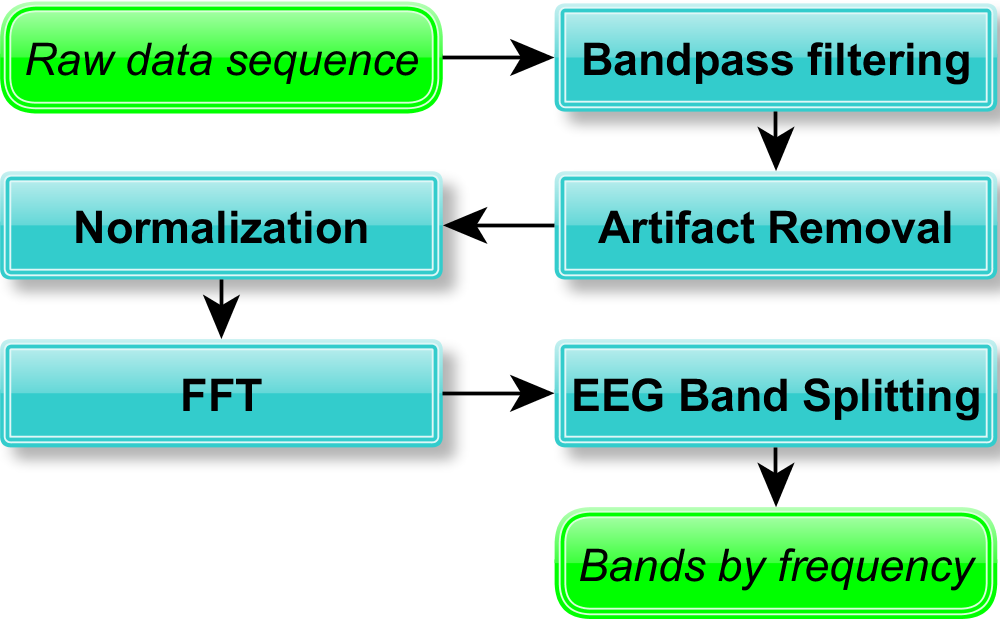
\includegraphics[width=\columnwidth]{data_processing_chain}
    \caption[Verarbeitungskette]{Die Signalsequenzen durchlaufen eine Verarbeitungskette \label{fig:data_processing_chain}}
  \end{center}
\end{figure}

Um Störungen zu eliminieren wurde das Signal zu Beginn außerhalb des Bereichs von 0.53Hz - 50Hz eliminiert. Dies war eine Empfehlung aus einer Antwort auf ResearchGate \cite{resGate} und zeigt bei Tests gute Ergebnisse. Werte über 50Hz abzuschneiden macht Sinn, da diese Werte für die Müdigkeitserkennung keine Rollen spielen ($\beta-$ und $\gamma$-Wellen). Signale unterhalb 0.53Hz ebenfalls zu entfernen hängt mit elektrischen Störungen zusammen. Der Bandpassfilter zentrierte das Signal zudem. 

Für die Anwendung wurde hierfür ein Buttworth-Filter\cite{Butterworth30} eingesetzt. Gleichung \ref{eq:butterworth} zeigt die Übertragungsfunktion mit $A_0$: Gleichspannungsverstärkung, $\Omega = \frac{f}{f_g}$: auf Grundfrequenz normierte Frequenz und $n$: Ordnung des Filters.  Der Butterworth-Filter verläuft nahe Eins im gewünschten Bereich, fällt an den Grenzen ab und stellt sicher, dass das Signal an den Grenzen um $\frac{1}{\sqrt{2}} \approx 0.7071$ gemindert wird. Je höher die Ordnung, desto steiler geht die Funktion durch die angegebenen Grenzen. Als analoger Filter lässt er sich gut in Hardware realisieren.

\begin{equation} \label{eq:butterworth}
\left|\underline{A}\right|^2 = \frac{A_0^2}{1+ k_{2n} \Omega ^{2n}}
\end{equation}

Bei der Analyse der Histogramme der Signalwerte, zeigte sich eine Häufung der Amplituden im Bereich von -100 bis 100. Werte außerhalb dieses Bereichs wurden als Artefakte angesehen und herausgefiltert bzw. als ungültig markiert\rawHisto

Die gefilterten Signale werden dann auf einen Bereich von -1 bis 1 normalisiert, dazu werden sie durch den jeweiligen Maximalwert bzw. Betrag des Minimalwertes geteilt (in diesem Fall 100). Dieses Vorgehen stellt sicher, dass die absolute Amplitude keinen Einfluss auf die Gewichtung im Klassifikator hat. Zudem wird die Datenmenge wiederum reduziert. 

Im letzten Schritt wird das Signal in seine Frequenzbänder (EEG-Bänder) unterteilt. Dazu wird es aus dem Zeitbereich in das Frequenzspektrum  überführt und bestimmte Frequenzbereiche extrahiert. Diese EEG-Bänder gliedern sich in folgende Bereiche und werden nach griechischen Buchstaben benannt: $\delta$ : 0,5 - 4Hz, $\theta$ : 4 - 8Hz, $\alpha$ : 8 - 13Hz, $\beta$ : 13 - 30Hz, $\gamma$ : ab 30Hz. Die Frequenzbereiche sind nicht einheitlich definiert und variieren unter Umständen, sie sind aus Empfehlungen der IFCN entnommen \cite{ifcn}. Den Frequenzbändern werden verschiedene Eigenschaften zugesprochen \cite{lei2011,Lv2010,Gundel1992}. Delta-Wellen treten bei Erwachsenen häufig in der traumlosen Tiefschlafphase auf. Theta-Wellen zeigen sich bei Schläfrigkeit und leichtem Schlaf. Mit leichter Entspannung und entspannter Wachheit (mit geschlossenen Augen) werden Alpha-Wellen assoziiert. Beta-Wellen treten während der REM-Schlafphase oder unter Einwirkung von Psychopharmaka auf. Gamma-Wellen gehen häufig mit starker Konzentration oder Meditation einher.

Um die einzelnen Frequenzbänder zu erhalten wird eine Fast-Fourier-Transformation \cite{Bochner_1} durchgeführt. \wavelet
 Die Fourier-Transformation bildet ein aperiodische, kontinuierliches Signal auf ein diskretes, periodisches Frequenzspektrum ab. Um die Frequenzbänder zu erhalten, wird das Ergebnis auf die gewünschten Frequenzen reduziert\fftExample
